% Innehållet i Vasungavisor 2010
%
% Kapitel "I Högan Nord"

\songchapter{Auld Acquaintance}
\begin{figure}[!b]
\begin{center}
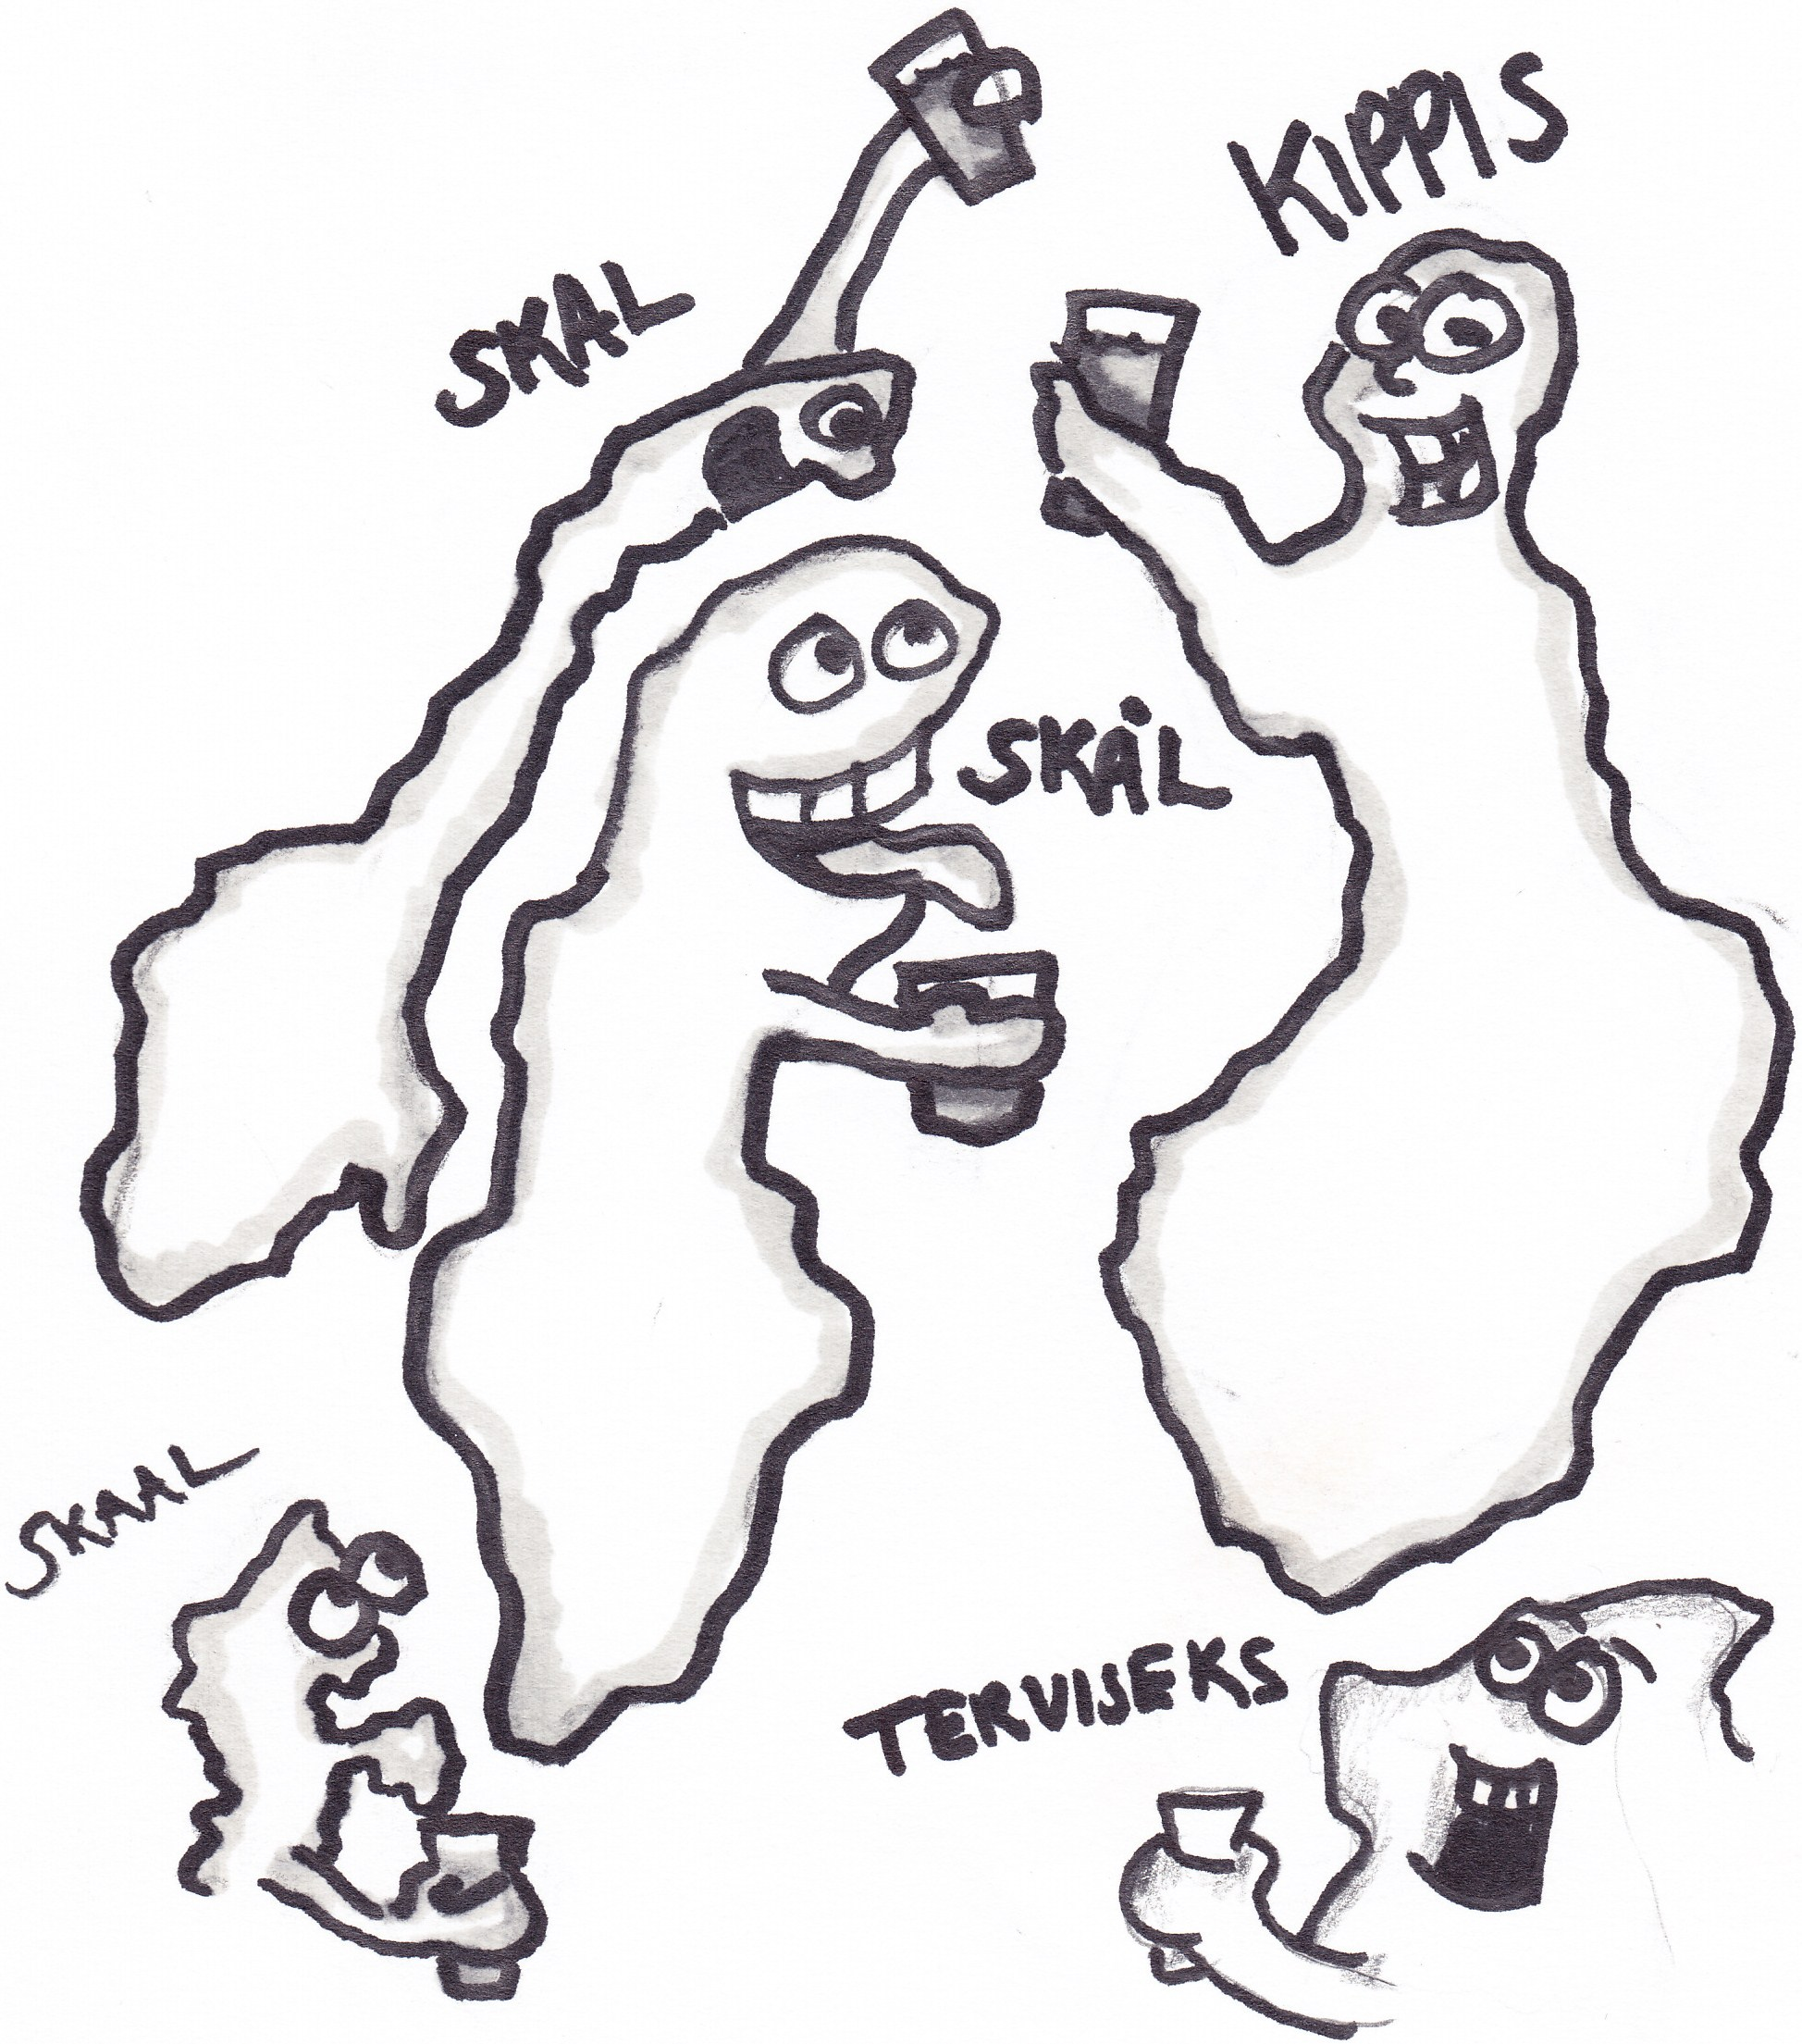
\includegraphics[width=6cm]{../bilder/auld.jpg} 
\end{center}
\end{figure}
\clearpage
% Innehållet i Vasungavisor 2010

\beginsong{Jag trivs bäst i Österbotten}[
	by={Claus Stolpe, Kimmo Rautanen},
	sr={Jag trivs bäst i öppna landskap}]
  
\beginverse*
Jag trivs bäst i Österbotten.
Opp i Pampas vill jag bo
tre månader om året
så att levern kan få ro.
Jag mår bäst en lördagsafton
på väg till någon dans
till en paviljong vid havet
opp i Pampas någonstans.
Där brygger jag mitt kaffe själv
och blandar det med hembränd sprit
och dricker det med välbehag
med gris från bageri't. 
Jag trivs bäst i österbotten
Opp i Pampas vill jag bo. 
\endverse

\beginverse*
Jag trivs bäst när blodet svallar
och fyllona ger skrin
när stranden fylls av tomglas
och heavypotpurrin.
När det klar och det rena
få rinna som det vill
och ordningsmännen tittar bort
och länsman har gått vill. 
Där raglar jag så sött omkring
och somnar sen mot närmsta sten
där redan farfar slocknade
nån gång för länge sen.
Jag trivs bäst i Österbotten
Opp i Pampas vill jag bo.
\endverse

\endsong

\clearpage
% Innehållet i Vasungavisor 2010

\beginsong{I Norrland växer det}[
  sr={I Apladalen i Värnamo}]
  
\beginverse*
I Norrland växer det tallar höga.
Att dom är höga det båtar föga,
för en vacker dag faller dom omkull
allt för den eviga törstens skull!
\endverse
\endsong
\begin{figure}[!b]
\begin{center}
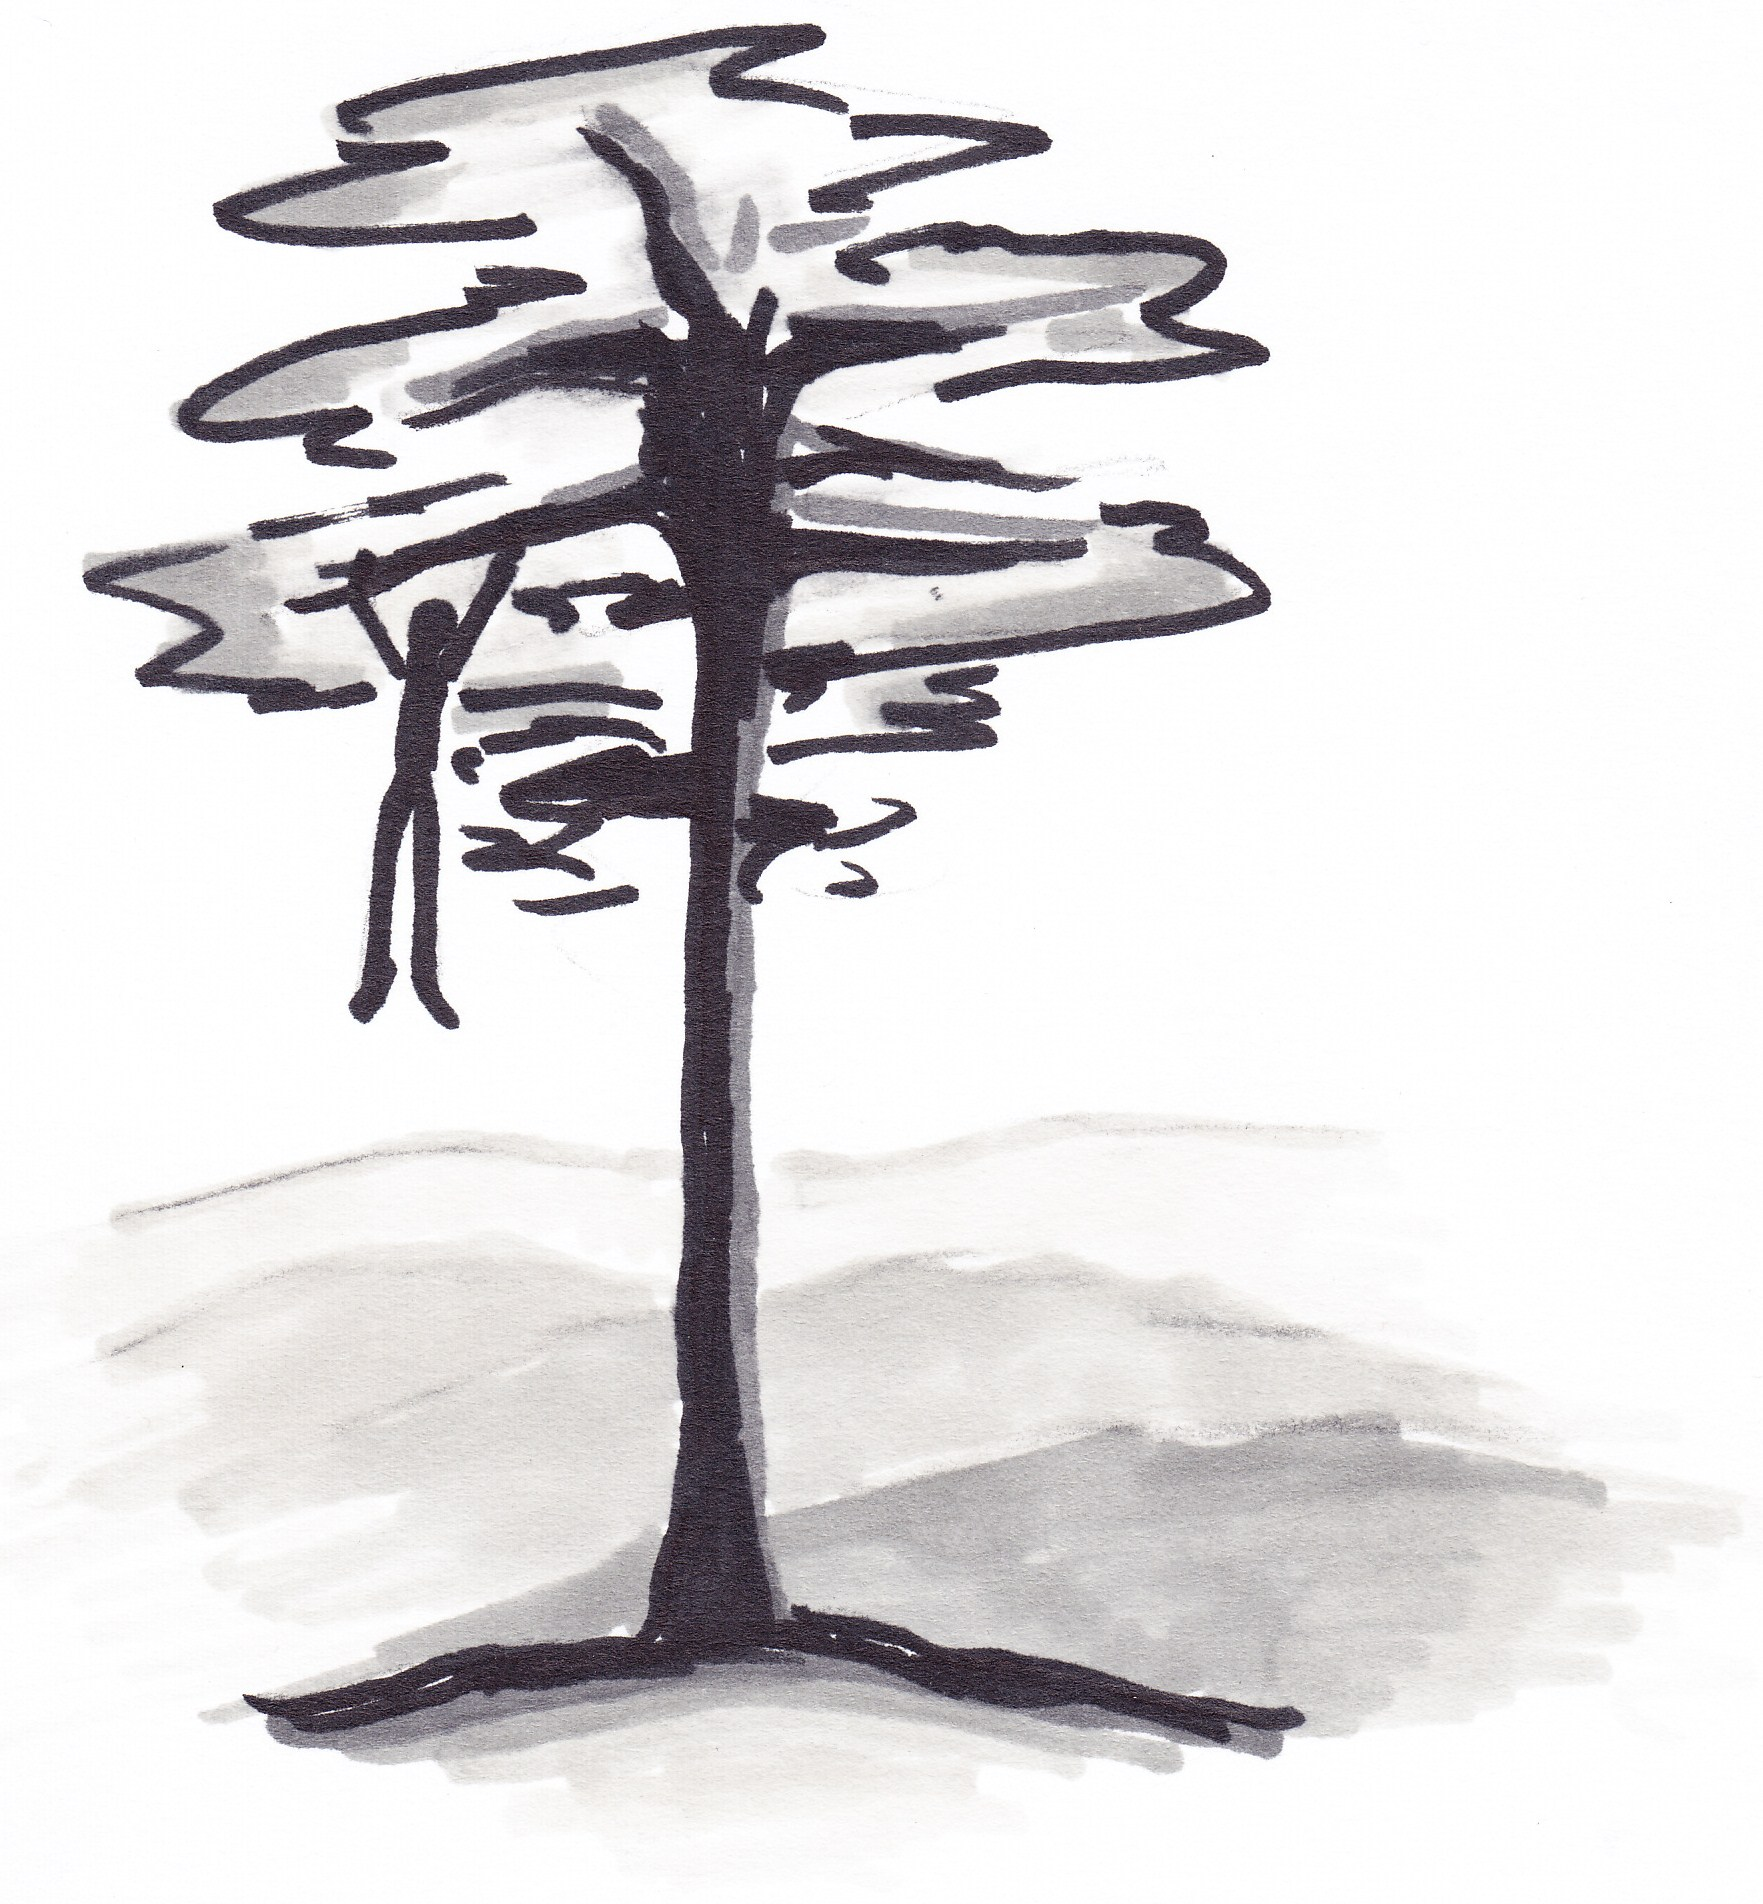
\includegraphics[width=4cm]{../bilder/inorrland.jpg} 
\end{center}
\end{figure}
\clearpage
% Innehållet i Vasungavisor 2010

\beginsong{Vi kom' från Norrland}[
	sr={Vi bor på landet}]
  
\beginverse*
Vi kom' från Norrland. Vi käkar myggen
som vi fångar på kalhyggen.
Och vi lägg' han uppå smörgåsen
som vi ät' med laxen,
renen,
sillen,
smöre,
nubben,
kåtan,
pölsan,
päran,
fjälle,
filen,
Åkes hammock
och det gör vi varje dag. 
\endverse

\beginverse*
Han hette Åke och var fån Tåsjö.
Han had' en gris som var fån Blåsjö.
Som han lade uppå smörgåsen
som han käkade med laxen ....
... och det gör han varje dag. 
\endverse

\beginverse*
Sen har vi Herman, ham kom' fån Böle.
Han hade Norrlands minsta hemman.
Han gick å kratte, och kärringa skratte
så han la'na på smörgåsen
och han käka'na med laxen...
...och det gör han varje dag. 
\endverse

\beginverse*
Sen har vi Göran, han kom fån Pite'
han har ingen hjärna men det skit' vi i.
För han la den uppå smörgåsen
som han åt med laxen....
...och det gör han varje dag. 
\endverse
\endsong

\clearpage
% Innehållet i Vasungavisor 2010

\beginsong{Kalmarevisan}

\beginverse*
Uti Kalmare stad,
ja, där finns det ingen kvast
förrän lördagen.
Hej dick,
hej dack.
Jag slog i
och vi drack.
Hej dickom dickom dack,
hej dickom dickom dack.
För uti Kalmare stad,
ja, där finns det ingen kvast
förrän lördagen.
\endverse

\beginverse*
När som kvasten kommer in
kommer viskorna med.
Var du säker på de'!
Hej dick ...
\endverse

\beginverse*
När som bonden kommer hem
kommer bondekvinnan ut
och är ful i sin trut.
Hej dick ...
\endverse

\beginverse*
Var är pengarna du fått?
Jo, dom har jag supit opp!
Uppå Kalmare slott.
Hej dick ...
\endverse

\beginverse*
Jag skall mäla dig an
för vår kronbefallningsman.
Och du skall få skam.
Hej dick ...
\endverse

\beginverse*
Kronbefallningsmannen vår
satt på krogen i går
och var full som ett får.
Hej dick ...
\endverse

\beginverse*
Vad skall bonden ha till mat
sura sillar och potat
de' blir sillsallat.
Hej dick ...
\endverse
\endsong

\begin{figure}[!b]
\begin{center}
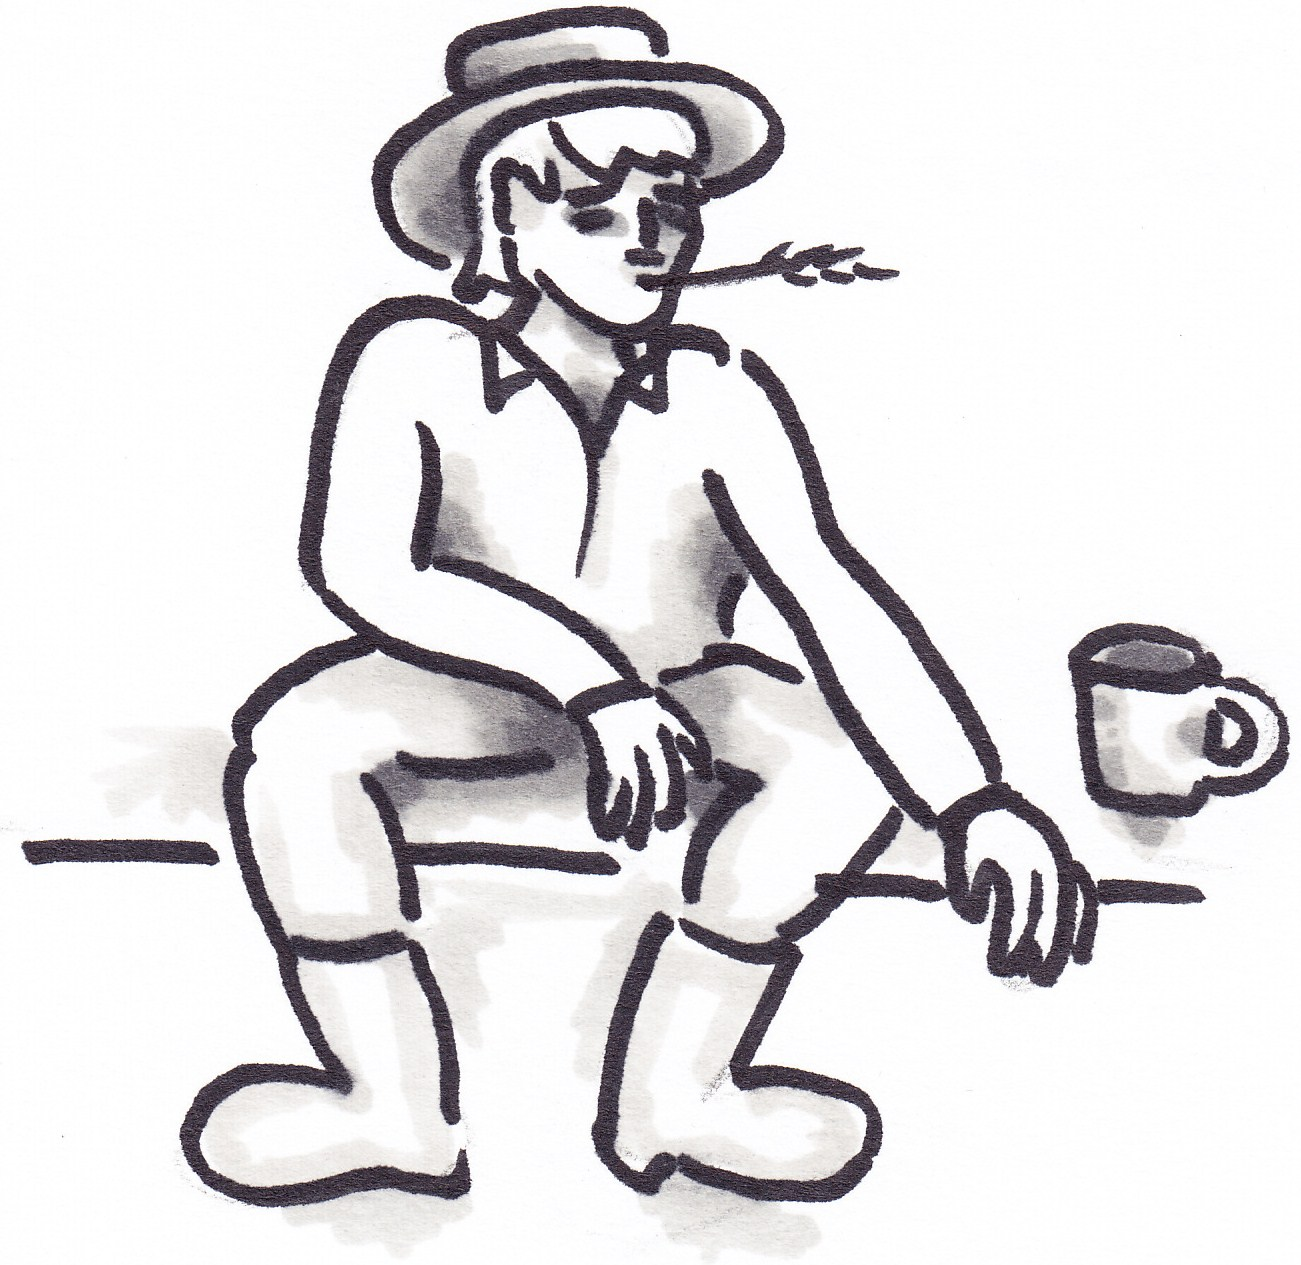
\includegraphics[width=4cm]{../bilder/bonde.jpg} 
\end{center}
\end{figure}
\clearpage
% Innehållet i Vasungavisor 2010

\beginsong{Lossis nimega gradesko}[
	by={Viktor von Scheffel}]
  
\beginverse*
Lossis nimega Gradesko,
kaugemal kui Temesvar,
istus vahva vürst Bibesko, Bibesko!
Serbia hall hospodar. 
\endverse

\beginverse*
Mida tegi vürst Bibesko,
Serbia hall hospodar,
lossis nimega Gradesko, Gradesko!
kaugemal kui Temesvar?
\endverse

\beginverse*
Slivovitši jõi Bibesko,
Serbia hall hospodar,
lossis nimega Gradesko, Gradesko!
kuni purjus oli vaar.
\endverse
\endsong

\clearpage
\beginsong{Me mõtted on priid}[
	by={August Anni}]

\beginverse
Me mõtted on priid,
kes suudaks neid köita?
Kes vägev on nii,
et vangi meid heita?
Ka vanglas ja vaevas
meil lahti on taevas.
:,: Kõikvõimsad me nii —
Me mõtted on priid. :,: 
\endverse

\beginverse
On elada rõõm
kesk päikese kulda,
On harida rõõm
maad emakest mulda.
Ja kannatust kanda
ja ohvriks end anda.
:,: Kõikvõimsad me nii —
Me mõtted on priid. :,: 
\endverse

\beginverse
Kõik muu meil ükskõik,
mis ise m'ei taha.
Meist enestest kõik,
kas hää see või paha.
Me süda ja silmad
need loovad maailma.
:,: Kõikvõimsad me nii —
Me mõtted on priid. :,: 
\endverse
\endsong
\clearpage
% Innehållet i Vasungavisor 2010

\beginsong{En dansk aquavit}[
  by={Knud Vad Thomsen},
  index={Ren som en jomfru}]
  
\beginverse*
Ren som en jomfru og stark som en bejler.
Hed som det hjarte, der hamrer mod dit.
Kølig som kilden, dervårhimlen spejler:
Sådan min ven, er en dansk aquavit.
Sådan min ven, er en dansk aquavit.
\endverse
\endsong
\begin{figure}[!b]
\begin{center}
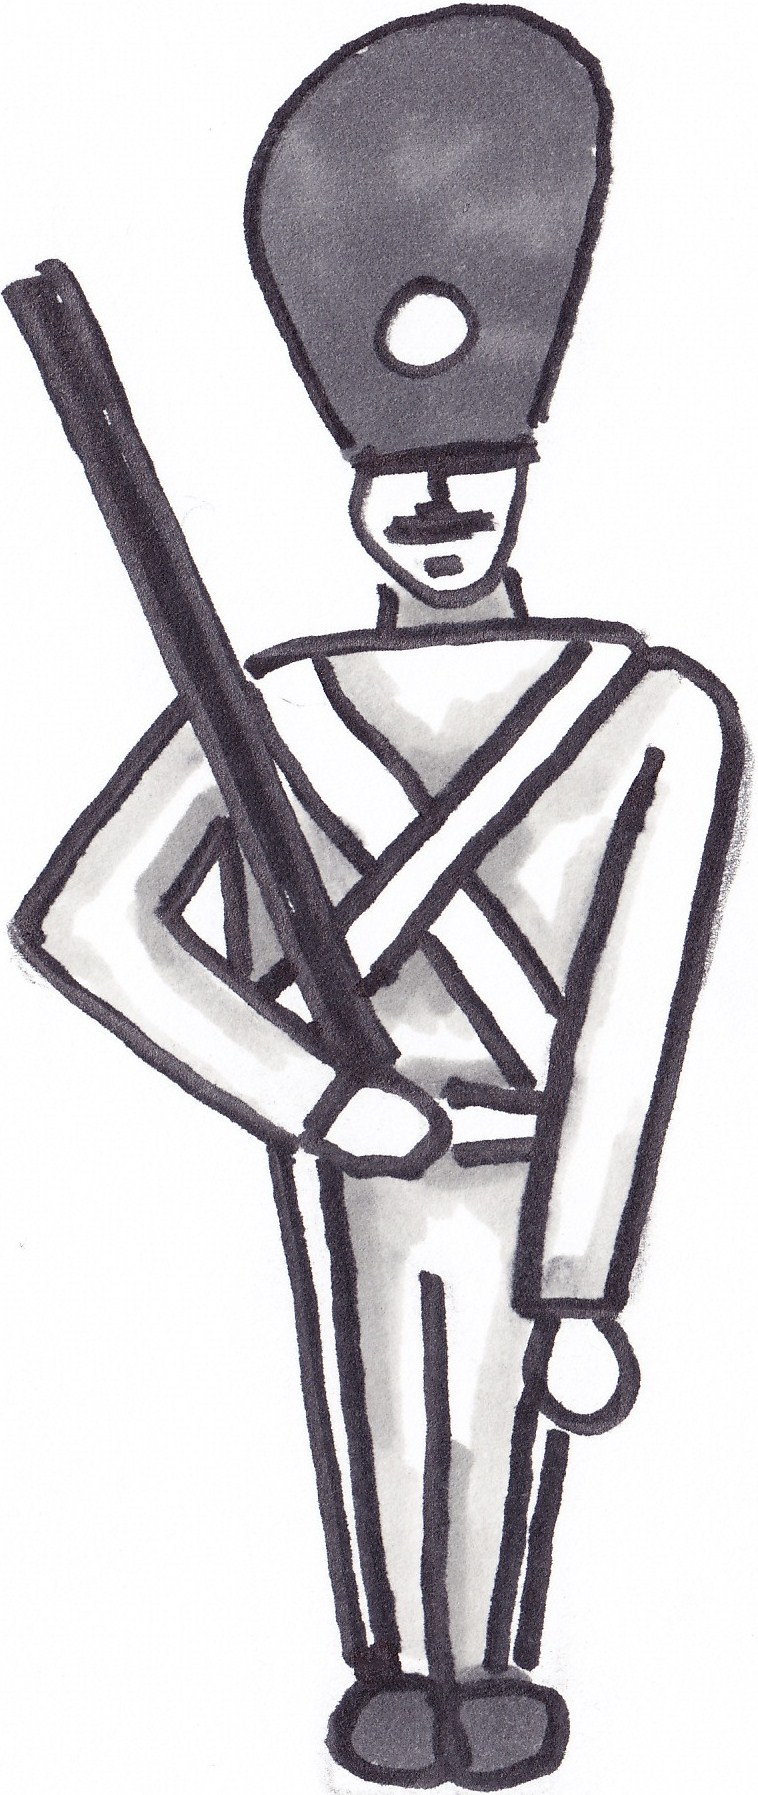
\includegraphics[width=25mm]{../bilder/dansk.jpg} 
\end{center}
\end{figure}
\clearpage
\beginsong{Viina painaa}[
	by={Marjatta Pokela},
		sr={Käki kukkuu kuusikossa}]

\beginverse
Viina painaa, viina painaa,
viina painaa aina.
Kauppakassissa lauantaina
ja päässä sunnuntaina.
\endverse

\beginverse
Viina maistuu, viina maistuu,
viina maistuu aina.
Arkipäivän askareissa
ja vielä sunnuntaina.
\endverse

\beginverse
Vesi loppuu, vesi loppuu,
vaan ei lopu viina.
Veden puute on paha juttu,
mutt' viinan puute on piina!
\endverse
\endsong
\clearpage
% Innehållet i Vasungavisor 2010

\beginsong{Jos eukkosi kieltää}
  
\beginverse*
Jos eukkosi kieltää sua juomasta,
niin juo, niin juo.
Jos kieltää sua viinoja tuomasta,
niin tuo, niin tuo.
Mutt' juomasta älä sinä milloinkaan lakkaa,
vaan hanki sinä itselles' parempi akka.
Ja juo ja laula, ja juo ja laula,
ja juo ja laula, ja juo ja laula...
\endverse

\beginchorus
Trink, trink, Brüderlein trink
lass doch die Sorgen zu Haus
trink, trink, Brüderlein trink
leere dein Glas mit mir aus
Meide den Kummer und meide den Schmertz
dann ist das Leben ein Schertz.
Kauf dir ein Auto und fahr gegen Baum
dann ist das Leben ein Traum
\endchorus

\beginverse*
Upseerit sotia taistelee,
ja juo, ja juo,
ja teltassa viinoja maistelee,
ja juo, ja juo.
Kun taistelun melskeessä pyssyt ne paukkaa,
niin upseerit välillä pullosta naukkaa,
ja juo ja laulaa ...
\endverse

\beginchorus
Trink, trink, Brüderlein trink...
\endchorus

\beginverse*
Maisterit koulussa opettaa,
ja juo, ja juo,
ja illalla tuntinsa lopettaa,
ja juo, ja juo.
Kun päivällä saksaa ja matikkaa jauhaa,
niin illalla raitilla räyhää ja pauhaa,
ja juo ja laulaa ...
\endverse

\beginchorus
Trink, trink, Brüderlein trink...
\endchorus

\endsong

\clearpage
% Innehållet i Vasungavisor 2010

\beginsong{Trink, Trink}
  
\beginverse*
Trink, trink, Brüderlein, trink,
lass doch die Sorgen zu Haus!
Trink, trink, Brüderlein, trink,
bald ist das Leben aus!
/: Meide den Kummer und meide das Schmerz,
dann ist das Leben ein Scherz :/
\endverse

\beginverse*
/: Meide die Weiber und meide das Bier,
dann wird ein Sportmann aus Dir :/
\endverse

\beginverse*
/: Heirat in Sommer und Scheide in März,
dann ist das Leben ein Scherz :/
\endverse

\beginverse*
/: Kauf dir ein Auto, fahr gegen ein Baum
so wird das Leben ein Traum :/
\endverse

\endsong

\begin{figure}[!b]
\begin{center}
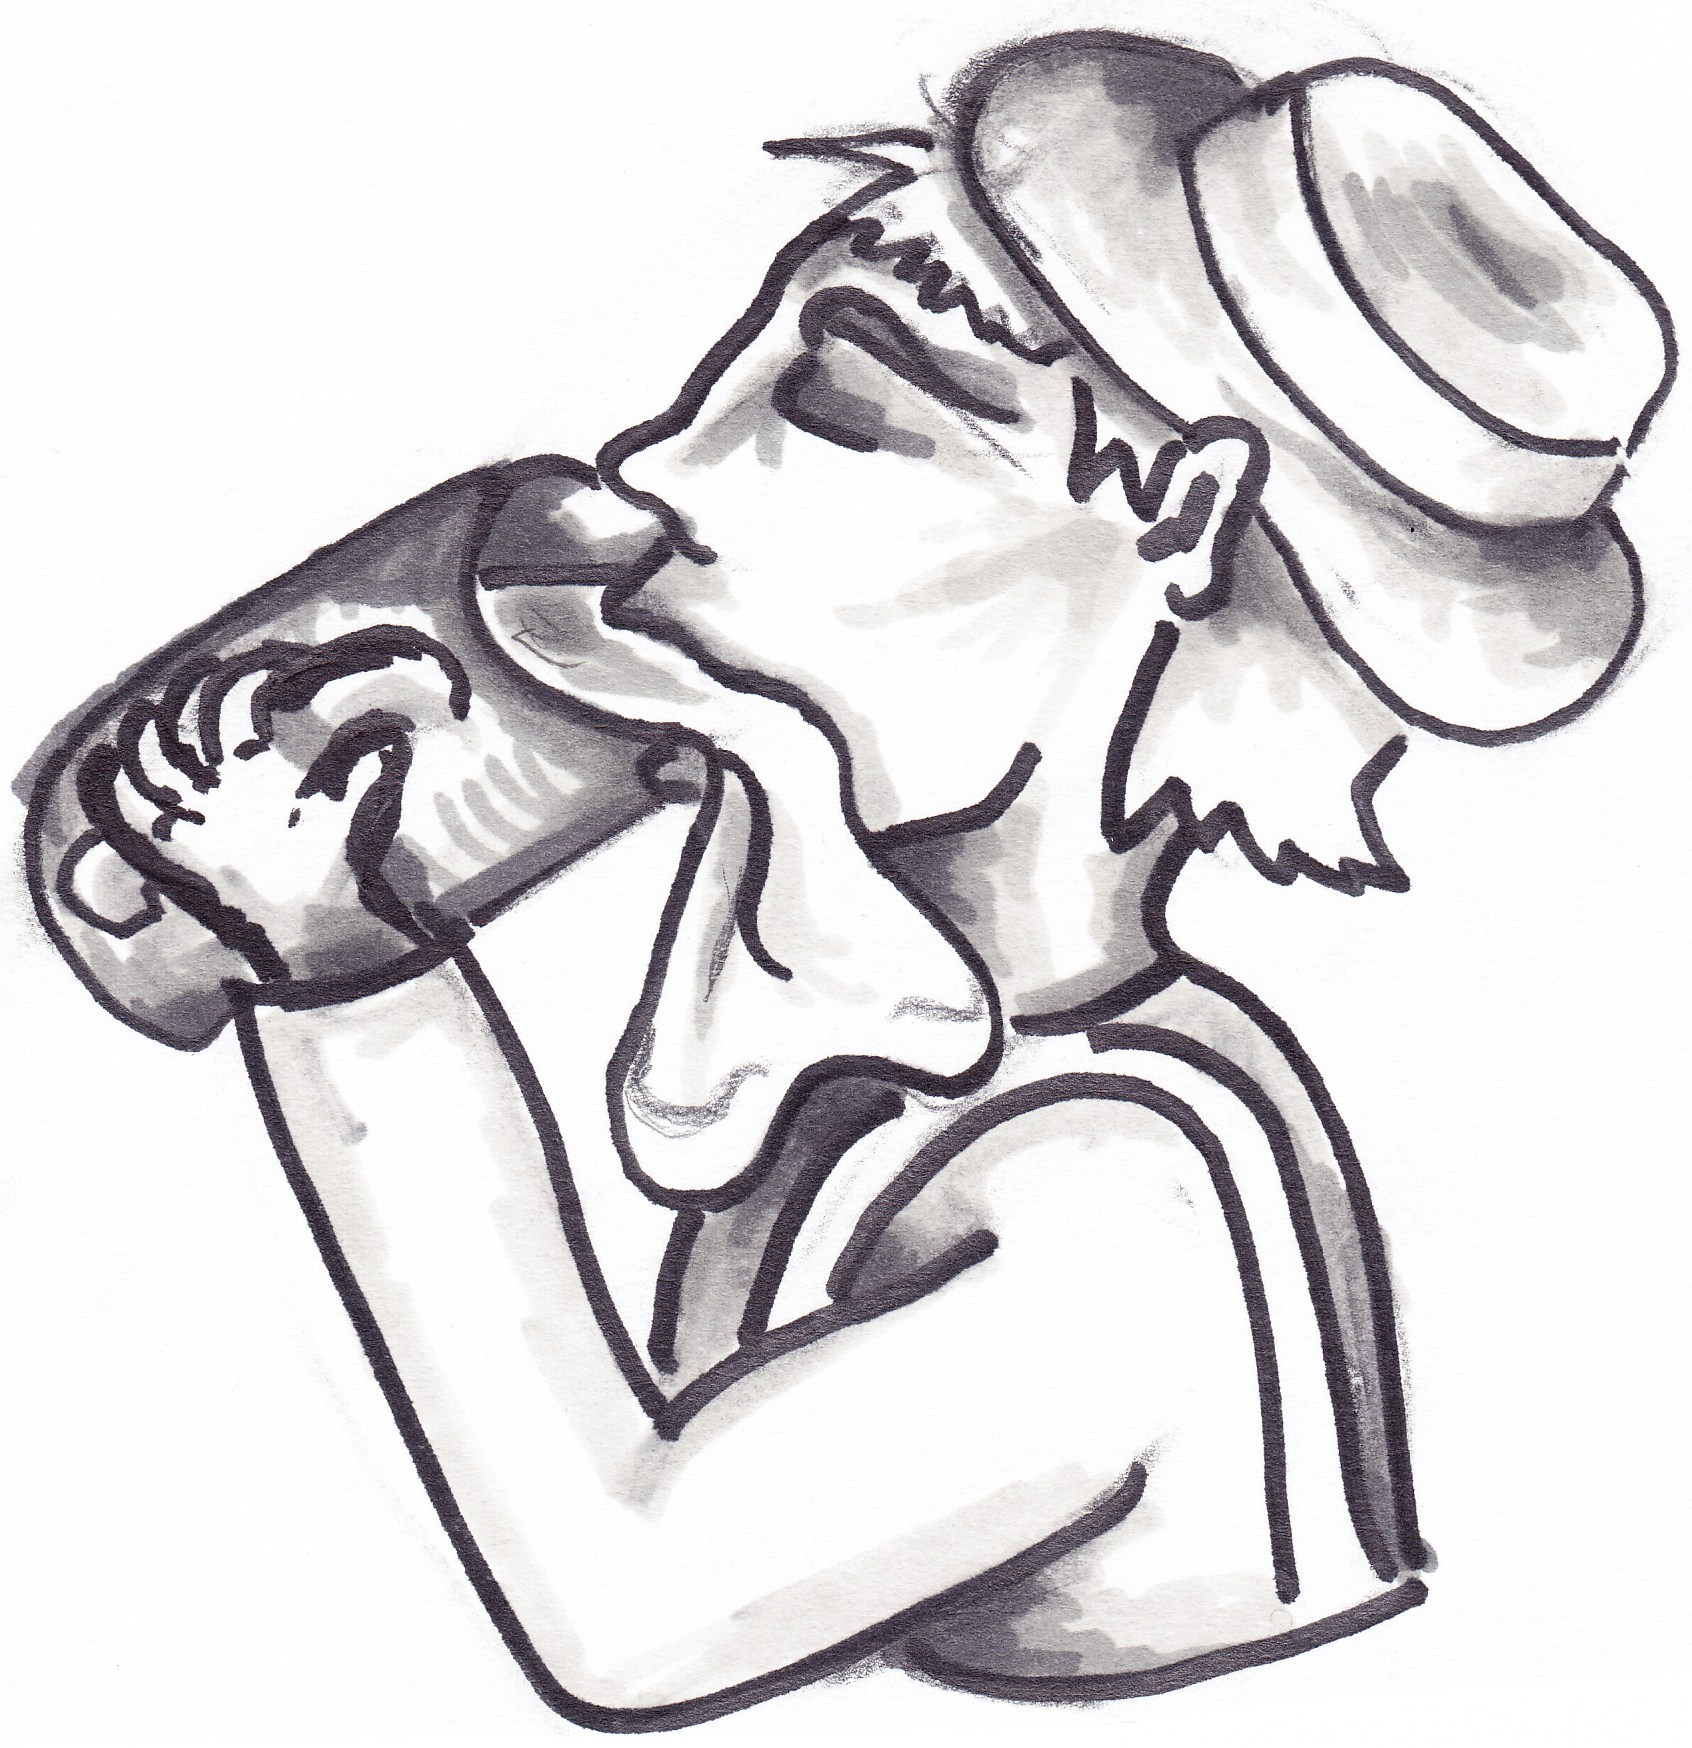
\includegraphics[width=3cm]{../bilder/trinktrink.jpg} 
\end{center}
\end{figure}
\clearpage
% Innehållet i Vasungavisor 2010

\beginsong{Urbummellied}[
	by={Carl Maria von Weber},
	index={Studio auf einer Reis}]
  
\beginverse*
Studio auf einer Reis'.
Juchheidi, juchheida.
Ganz famos zu leben weiß.
Juchheidi, heida!
Immer fort durch Dick und Dünn
schlendert er durch's Dasein hin.
\endverse

\beginverse*
Hat der Studio auch kein Geld.
Juchheidi, juchheida.
Ist er drum nicht schlecht bestellt.
Juchheidi, heida!
Manches feinste Pfäffelein,
ladet ihn zum Frühstück ein.
\endverse

\beginverse*
Kehren wir in's Wirtshaus ein.
Juchheidi, juchheida.
Trinken wir stets Bier und Wein.
Juchheidi, heida!
Alle Mädel für uns glühn,
denn wir tragen schwartz-blau-grün.
\endverse

\beginverse*
Bayrisch Bier und Leberwurst.
Juchheidi, juchheida,
Und ein Kind mit voller Brust.
Juchheidi, heida!
Und ein Glas Crambambuli,
Donnerwetter Paraplui!
\endverse
\endsong

\clearpage
% Innehållet i Vasungavisor 2010

\beginsong{So troll’n wir uns}[
	by={Carl Zuckmayer},
	sr={Så lunka vi}]
  
\beginverse*                                        
So troll'n wir uns ganz fromm und sacht
von Weingelag und Freudenschmaus,
wenn uns der Tod ruft: Gute Nacht,
Dein Stundenglas rinnt aus.
Wer heut noch frech den Schnabel wetzt
und glaubt, ein großer Herr zu sein,
pass auf, der Schreiner hobelt jetzt
grad schon an deinem Schrein.
\endverse

\beginchorus
Scheint das Grab dir tief und dumpf sein Druck:
Alavott, so nimm noch einen Schluck,
und noch einen hinterher,
und rasch noch zweie, dreie mehr,
dann stirbt sich’s nicht so schwer.
\endchorus

\beginverse*
Der nach des Andren Liebsten schielt
und doch sich fühlt als Nobelmann,
pass auf! Dem Spielmann, der dir spielt,
springst du ins Grab voran!
Und du, der toll vor Eifersucht
zerschmiss einst jedes Glas im Saal –
wenn dich der Tod im Bett besucht –
hoch lebe dein Rival!
\endverse

\beginchorus
Scheint das Grab dir tief...
\endchorus

\beginverse*
Was hilft's, wenn du vor Wut auch spuckst,
der Tod ist keiner Münze feil.
Von jedem Schlückchen, das du schluckst,
schluckt schon der Wurm sein Teil.
Ob niedres Pack, ob hohe Herrn –
am Ende sind wir Brüder doch:
dann leuchtet uns der Abendstern
ins gleiche finstre Loch.
\endverse

\beginchorus
Scheint das Grab dir tief...
\endchorus
\endsong

\clearpage
% Innehållet i Vasungavisor 2010

\beginsong{Auld lang syne}

\beginverse*
Should auld acquaintance be forgot,
and never brought to mind?
Should auld acquaintance be forgot,
and days o' auld lang syne. 
\endverse

\beginchorus
For auld lang syne, my dear,
for auld lang syne.
We'll tak a cup o' kindness yet,
for auld lang syne.
\endchorus

\beginverse*
And here's a hand, my trusty friend,
and gie's a hand o' thine!
We'll tak a right guid willy waught,
for auld lang syne. 
\endverse

\beginchorus
For auld lang syne, my dear,
for auld lang syne.
We'll tak a cup o' kindness yet,
for auld lang syne.
\endchorus
\endsong

\clearpage
% Innehållet i Vasungavisor 2010

\beginsong{What should we do with the drunken sailor?}
  
\beginverse*                                        
What should we do with the drunken sailor 
What should we do with the drunken sailor
What should we do with the drunken sailor 
early in the morning?
\endverse

\beginchorus
Ho-ray and upp she rises,
ho-ray and upp she rises,
Ho-ray and upp she rises,
early in the morning!
\endchorus

\beginverse*
Put him in the long boat until he's sober...
\endverse

\beginchorus
Ho-ray and upp she rises...
\endchorus

\beginverse*
Pull out the plug and wet him all over...
\endverse

\beginchorus
Ho-ray and upp she rises...
\endchorus

\beginverse*
Put him in a bed with the captain's daughter...
\endverse

\beginchorus
Ho-ray and upp she rises...
\endchorus
\endsong

\clearpage
\beginsong{Kuka helvetti}[,
		sr={Polonaise}]

\beginverse
Kuka helvetti heitti kiven mun
viinapulloon? (x 4)
\endverse

\beginverse
Vem i helvete kasta' sten på min
flaska brännvin? (x 4)
\endverse

\beginverse
Who the hell threw this bloody stone at my
whisky bottle? (x 4)
\endverse

\beginverse
Wer zum Teufel warf ein Stein zu mein
Flasche Rheinwein? (x 4)
\endverse

\beginverse
Kes kurat viskas kive minu
viinapudelisse? (x 4)
\endverse

\beginverse
Saku Sammakko heitti kiven mun
viinapulloon! (x 4)
\endverse
\endsong